% CiteLume manuscript for the Journal of Biomedical Informatics (Elsevier elsarticle template).
% Build: latexmk -pdf main.tex   (from this folder)
% Every item still to be filled in is marked \TODO{...} (owner) or \PENDING{...} (a result not yet available);
% `grep -n "TODO\|PENDING" main.tex sections/*.tex` lists them.
\documentclass[preprint,12pt,authoryear]{elsarticle}

\usepackage[T1]{fontenc}
\usepackage[utf8]{inputenc}
\usepackage{lmodern}
\usepackage{amsmath}
\usepackage{graphicx}
\usepackage{booktabs}
\usepackage{tabularx}
\usepackage{multirow}
\usepackage{xcolor}
\usepackage{lineno}
\usepackage[hidelinks]{hyperref}
\usepackage{tikz}
\usetikzlibrary{positioning,arrows.meta,fit,backgrounds,calc}

\newcommand{\TODO}[1]{\textcolor{red}{[TODO: #1]}}
\newcommand{\PENDING}[1]{\textcolor{orange}{[PENDING: #1]}}
\newcommand{\tool}{CiteLume}

\journal{Journal of Biomedical Informatics}
\linenumbers

\begin{document}

\begin{frontmatter}

\title{Protocol-first, replayable study selection for LLM-assisted evidence synthesis:
design of \tool{} and a pre-registered evaluation on Cochrane intervention reviews}

\author[aff1]{Bhargava \TODO{family name}\corref{cor1}}
\ead{\TODO{e-mail}}
\cortext[cor1]{Corresponding author.}
\address[aff1]{\TODO{affiliation, or ``Independent researcher'', city, country}}
% ORCID: \TODO{ORCID}

% Structured abstract (JBI: Objective, Methods, Results, Conclusion; about 300 words -- \TODO{confirm limit in the
% Guide for Authors}). Currently about 300 words.
\begin{abstract}
\textbf{Objective:} Tools that use large language models (LLMs) to find and select studies for literature reviews
can return different studies on repeated runs and rarely report how many of a review's studies they find. We
describe a design in which study selection is rule-based, stored and replayable, and the model's role is limited to
planning searches and screening against stated criteria, and we evaluate its recall and repeatability.

\textbf{Methods:} \tool{} turns a question into a review protocol, searches PubMed, Europe PMC, Semantic Scholar or
OpenAlex, bioRxiv/medRxiv and arXiv with search strings compiled by fixed rules (with MeSH headings), adds
citation searching, merges duplicates, applies eligibility rules and a published 100-point score and, for
systematic-style reviews, has a model screen titles and abstracts against the protocol's criteria. Every record and
decision is stored in a corpus from which the selection can be replayed. We evaluated it, under a protocol
registered before any data were loaded, on 33 Cochrane intervention reviews from CLEF TAR 2019 (11 development, 22
held-out test), freezing search and selection before test results were used.

\textbf{Results:} On the 22 test reviews, the candidate pool held a mean of 54\% (95\% CI 41--67\%) of each review's
included studies, and the selection 25\% (15--35\%); model screening kept 87\% (72--99\%) of the included studies it
saw. Of the 538 included studies not selected, 80\% were lost at search (49\% beyond the retrieval depth, 31\%
matched by no query). Selection replayed exactly from the stored records in 44 of 44 corpora; repeated screening of
the same records agreed with Cohen's $\kappa$ 0.91--0.94; halving or increasing the score weights by half changed
recall by at most 0.3 percentage points. \PENDING{claim accuracy: share of 200 cited sentences supported by the
cited studies (Session 8 annotation)}

\textbf{Conclusion:} Separating a replayable, rule-based selection from model-assisted search and screening makes
LLM-assisted study selection auditable and exactly reproducible from stored records. Recall is limited mainly by
search depth and query sensitivity, which shows where such tools need to improve and that they support, rather
than replace, a systematic search.
\end{abstract}

% Graphical abstract: \TODO{required at submission (separate file); draft from Fig. 1 and Fig. 2}


\begin{keyword}
systematic reviews \sep literature search \sep study selection \sep large language models \sep
reproducibility \sep PRISMA
\end{keyword}

\end{frontmatter}

\section{Introduction}
\label{sec:intro}

Systematic reviews answer questions about the effects of health interventions by finding, appraising and combining
every study that meets criteria set in advance \citep{higgins2023handbook,page2021prisma}. Finding and selecting
those studies is the most labour-intensive part: searches across several databases return thousands of records,
and two reviewers screen each one \citep{borah2017analysis,lefebvre2023searching}. Automating parts of this work
has been studied for two decades, mostly as text classification that ranks or filters records for human screeners
\citep{cohen2006reducing,omara2015using,marshall2019toward,vandeschoot2021open}.

Large language models (LLMs) have widened the scope of such tools from ranking records to writing search strings,
screening titles and abstracts, extracting data and writing the synthesis \citep{wang2023can,guo2024automated,
khraisha2024can,asai2024openscholar}. They also bring a problem that ranking models did not: the same question can
produce a different set of studies each time it is asked, because the model's plan, the database responses and the
model's judgements all vary between runs. Repeating the same data extractions with a commercial LLM research
assistant agreed on 90\% of the extracted values but on only 46\% of the supporting quotations and 30\% of the
reasoning \citep{lagisz2026elicit}. A review whose
included studies cannot be reproduced cannot be audited or updated, and recent guidance on the responsible use of
AI in evidence synthesis asks tool developers to report how their tools were evaluated, to keep people in control
of decisions, and to label tools without robust evaluation as such \citep{raise2026,jointstatement2025}.

Most evaluations of LLM-based tools report agreement with human screening decisions on a fixed set of records
\citep{guo2024automated,khraisha2024can}. Fewer measure the whole path from question to included studies: how many
of the studies a published review included would the tool have found, at which step are the others lost, and does
a repeat of the same run give the same result? These are the questions a reviewer needs answered before relying on
such a tool for a search, and they have a clear reference standard in the included studies of published
systematic reviews \citep{kanoulas2019clef}.

This paper describes \tool{}, an open-source tool that separates the two kinds of work. The parts where a model
helps but may vary (planning searches, screening against criteria, writing) are bounded and recorded, and the part
that decides which studies are included (merging duplicates, eligibility and ranking) follows fixed, published
rules applied to stored records, so that it can be replayed exactly. Our contributions are:
\begin{enumerate}
\item A \emph{protocol-first, replayable} design for LLM-assisted study selection: the review protocol is set
  before searching; search strings are compiled by fixed rules; the rule-based selection does not read the model's
  plan; every record, decision and model judgement is stored in a corpus with a content hash, from which the
  selection can be reproduced without searching again or calling a model (Section~\ref{sec:design}).
\item A \emph{pre-registered evaluation} on 33 Cochrane intervention reviews with a development and held-out test
  split, in which the measured code was frozen before test results were used, reporting recall at each stage,
  where included studies are lost, baselines, and the repeatability of each step (Sections~\ref{sec:eval}
  and~\ref{sec:results}).
\item An analysis of the trade-off this design makes: keeping the selection independent of the model makes it
  reproducible but costs recall when the rule-based reading of the question is poor
  (Section~\ref{sec:discussion}).
\end{enumerate}

\section{Design of \tool{}}
\label{sec:design}

\subsection{Principles}

\tool{} is a web application and Python library (FastAPI back end, React front end, MIT licence). Three principles
shape it:
\begin{enumerate}
\item \textbf{Protocol first.} A question is turned into a review protocol before anything is searched: the review
  type, the parts of the question (concepts) with their synonyms, the populations or places every study must name,
  and the eligibility criteria. The tool proposes a protocol from the question's own words; in the guided review
  the user confirms or edits each part. The protocol is stored with the results.
\item \textbf{A bounded role for the model.} A model may propose synonyms and search aspects, screen titles and
  abstracts against the protocol's criteria, extract study details and write the synthesis. It never writes search
  strings, and the rule-based steps that decide inclusion (duplicate merging, eligibility and ranking) do not read
  its output: they match studies against the concepts parsed from the question by fixed rules, so the same records
  give the same candidates with any model or none.
\item \textbf{Everything stored, selection replayable.} Each run is stored as a \emph{corpus}: every record the
  searches returned (before and after merging), the search plan and strings, the protocol, every eligibility and
  screening decision with its reason and the model's name, the selection protocol version and the code commit,
  under a content hash. A replay function re-runs the selection from the stored records alone, with no network
  and no model, and checks that it reproduces the included studies, in order, with the same hash.
\end{enumerate}
Figure~\ref{fig:pipeline} shows the pipeline. The full selection rules are published in the repository
(\texttt{docs/RANKING.md}, generated from the code) and summarised below; they are those of selection protocol
\texttt{citelume-selection/2.5}, the version evaluated.

\begin{figure}[t]
\centering
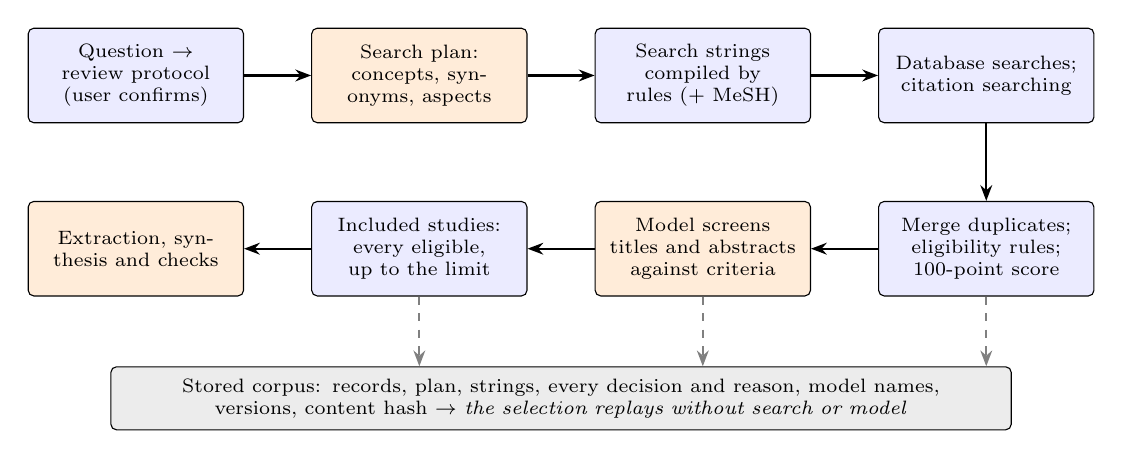
\begin{tikzpicture}[
  box/.style={draw, rounded corners=2pt, align=center, font=\scriptsize, minimum height=12mm, text width=25mm},
  model/.style={box, fill=orange!15},
  rule/.style={box, fill=blue!8},
  store/.style={draw, rounded corners=2pt, align=center, font=\scriptsize, fill=gray!15, text width=112mm,
    minimum height=8mm},
  arr/.style={-{Stealth[length=2mm]}, thick}]
\node[rule]  (q)       at (0,0)    {Question $\rightarrow$ review protocol (user confirms)};
\node[model] (plan)    at (3.6,0)  {Search plan: concepts, synonyms, aspects};
\node[rule]  (strings) at (7.2,0)  {Search strings compiled by rules (+ MeSH)};
\node[rule]  (search)  at (10.8,0) {Database searches; citation searching};
\node[rule]  (merge)   at (10.8,-2.2) {Merge duplicates; eligibility rules; 100-point score};
\node[model] (screen)  at (7.2,-2.2)  {Model screens titles and abstracts against criteria};
\node[rule]  (incl)    at (3.6,-2.2)  {Included studies: every eligible, up to the limit};
\node[model] (synth)   at (0,-2.2)    {Extraction, synthesis and checks};
\node[store] (corpus)  at (5.4,-4.1)  {Stored corpus: records, plan, strings, every decision and reason, model names,
  versions, content hash $\rightarrow$ \emph{the selection replays without search or model}};
\draw[arr] (q) -- (plan); \draw[arr] (plan) -- (strings); \draw[arr] (strings) -- (search);
\draw[arr] (search) -- (merge); \draw[arr] (merge) -- (screen); \draw[arr] (screen) -- (incl);
\draw[arr] (incl) -- (synth);
\draw[arr, dashed, gray] (merge.south) -- (merge.south |- corpus.north);
\draw[arr, dashed, gray] (screen.south) -- (screen.south |- corpus.north);
\draw[arr, dashed, gray] (incl.south) -- (incl.south |- corpus.north);
\end{tikzpicture}
\caption{The \tool{} pipeline. Orange steps may use a model; blue steps follow fixed rules. The rule-based steps that
decide which studies are candidates do not read the model's plan. Everything is stored in a corpus from which the
selection can be replayed.}
\label{fig:pipeline}
\end{figure}

\subsection{Search}

The question is reduced to one to three concepts that every relevant record must be about, each with synonyms;
a population or place named in the question is also required. With a model configured, the model proposes the
concepts, synonyms and four to six search aspects (for example mechanisms, adverse effects), and its concepts are
accepted only if the leading one is anchored in the question's words; otherwise fixed rules built for questions
written as review titles derive them. Search strings are then compiled by rules, never written by the model. For
each concept, PubMed is asked once how it maps the words to its controlled vocabulary, and the returned MeSH
headings and pharmacological actions are added as alternatives \citep{lefebvre2023searching}. Each database (PubMed
with its Europe PMC mirror, Semantic Scholar with OpenAlex as a fallback, bioRxiv/medRxiv and arXiv) receives a core
search (the concepts), a reviews search and one search per aspect. For systematic-style reviews the core PubMed
search can be paged deeper (500 records in the evaluation). After a first selection, the reference lists and citing
papers of up to 60 selected studies are fetched from Semantic Scholar (records linked to at least two are added),
and the reference lists of on-topic reviews set aside by the eligibility rules are added, as records identified by
other methods \citep{page2021prisma}. The strings, the number of records each PubMed search matched and how many
were retrieved are stored and shown.

\subsection{Selection}

Records for the same paper are merged by DOI, PubMed ID, arXiv ID or normalised title. Eligibility rules then
remove, each under its own reason: records outside a population or place the question names; records whose main
concept appears nowhere in the title, abstract or (for PubMed records) MeSH indexing; records that are not research
reports (corrections, retraction notices, protocols without results, meeting abstracts); and records outside the
protocol's years or designs. In a systematic-style review, reviews of all kinds are set aside and listed for the
discussion. Each remaining record receives a published 100-point score: relevance to the question (50 points:
concept matches in title and abstract, and BM25 wording overlap ranked among the candidates), study type (20 points,
from the database's publication type where available, otherwise from wording), citations per year ranked among the
candidates (15), recency (10) and the number of independent searches that found it (5).

For a quick answer the 20 highest-scoring studies are chosen with simple coverage rules (each search aspect is
represented; reviews limited to a share of places). For a systematic-style review there are no quotas: every
eligible primary study whose title or abstract addresses every part of the question is a candidate, and records
that match the main concepts but not every part go to model screening rather than being excluded by word matching.
The model then screens candidates in score order, in batches of 12, answering each protocol criterion as yes, no
or unclear for each record from its title and the first 420 characters of its abstract; a record is excluded only
if a criterion is clearly not met (``unclear'' never excludes). Screening continues until the study limit is filled
(150 in the evaluation), up to the larger of 240 records or twice the limit per review. Each decision is stored
with its reason and can be overturned by the user, with a recorded reason. Every exclusion is counted at its PRISMA
2020 stage for the flow diagram \citep{page2021prisma}.

\subsection{After selection}

A model extracts each included study's design, population, results and stated limitations (from open-access full
text where available) and writes a synthesis in which every sentence cites the studies it rests on; rule-based
checks compare figures and citations with the extracted details. Risk of bias is suggested only for studies with
open full text, each judgement resting on a quotation checked against the text and, for randomised trials, on the
RoB 2 algorithm \citep{sterne2019rob2}; it is presented as a suggestion for the reviewer and was not evaluated
against published judgements (Section~\ref{sec:limits}). This paper evaluates search and selection, the
repeatability of each step, and the accuracy of the written claims.

\section{Evaluation}
\label{sec:eval}

The evaluation protocol was written and committed on 18 November 2026, before any benchmark review was loaded or
run; changes were made only by dated amendments (Supplementary Material S2). The search methods are reported
following PRISMA-S \citep{rethlefsen2021prismas} (Supplementary Material S1). All code, stored corpora and results
are available (Section~\ref{sec:availability}).

\subsection{Benchmark}

We used the 40 Cochrane intervention reviews of CLEF eHealth TAR 2019, Task~2 \citep{kanoulas2019clef}, each with
the PubMed IDs of the studies the review included after full-text screening. Intervention reviews were chosen
because they ask effect questions, the kind \tool{}'s systematic-style protocol is built for; diagnostic and
prognostic topics were not used. Two reviews listed in both parts of the track were counted once, and five were
excluded by rules fixed beforehand (fewer than two included studies resolving to a PubMed record), leaving 33
reviews with 785 included studies (141 in the development set and 644 in the test set). The reviews were sorted by ID, shuffled with a fixed seed (20261118), and the first third formed the
development set (11 reviews); the other 22 formed the test set. Development reviews were used to change the
pipeline; test reviews were run only after the protocol was fixed.

\subsection{Runs}

Each review's title, unchanged, was the question; searches were limited to records published up to the year of the
review version CLEF used. Each test review was run in the systematic-style mode (Deep Research, PubMed core search
500 records deep, citation searching and review reference lists on, study limit 150) and in the quick-answer mode.
The model for planning, screening and analysis was NVIDIA Nemotron 3 Ultra (\url{nvidia/nemotron-3-ultra-550b-a55b})
through OpenRouter, on its free endpoint for the systematic-style runs and its paid endpoint for the quick-answer
runs (total cost 0.77~USD). All 22 searches in each mode were planned by the model. Every run went through a batch
runner that stores the corpus, result, timings, model and code commit, and fails a run in which more than 5\% of the
records due for screening were not screened.

\subsection{Freezing the measured code}

Search and selection were frozen at selection protocol 2.5 (code commit 47e40ef, git tag
\texttt{eval-freeze-2.5}) on 23 November 2026, after the systematic-style test runs and before any further run
(protocol amendment, Supplementary Material S2). The hashes of the frozen files and functions are recorded and
checked by an automated test, so any later change to search or selection fails the test suite until it is
recorded as a post-freeze change. One post-freeze fix was made (a bioRxiv connector error that did not occur in any
evaluation run).

\subsection{Measures}

The primary measure was \emph{pool recall}: the share of a review's included studies present in the candidate pool
after duplicate merging. Secondary measures were the share in the top 20 and top 60 of the screening order, the
share selected after model screening, screening sensitivity (included studies kept by the model, of those it
screened) and precision, and the loss of included studies at each stage (search, merging, eligibility, screening and
study limit). A study counted as found when a record carried its PubMed ID or DOI (case-insensitive) or, for records
with neither, the same normalised title. Each measure was computed per review and summarised as the mean with a 95\%
bootstrap confidence interval over reviews (10,000 resamples, seed 20261118) and the median, over all reviews and
over the reviews with at most 60 included studies. Baselines ranked the same pools by BM25 against the question, by
citation count alone, and at random.

\subsection{Repeatability and sensitivity}

On the stored test corpora we measured (E2a) whether the selection replays exactly from the stored records;
(E2b) the agreement of model screening with itself, by screening a sample of 1,638 records (up to 96 per review,
every screened included study first) three more times with the same model and prompt; (E2c) the variation in
records found when each question is searched twice more; (E2d) the effect of model planning, by repeating the
searches with rule-based planning and re-planning each question three times with the model; and (E3) the
sensitivity of the selection to its constants, by setting each score weight and cap to half and one and a half
times its value and comparing the selections (Jaccard overlap) and recall.

\subsection{Component checks}

We checked the study-type classifier against the publication types PubMed indexers assigned to 26,114 records from
the evaluation runs, with those types removed so the classifier had to rely on wording, as it does for most
preprint and some Semantic Scholar records. We sampled 100 duplicate merges from the test runs (1,351 merges on title
alone and 99 merges of records sharing an identifier with differing titles), weighted to the harder kinds, for a
person to judge whether each pair was the same study \PENDING{merge check result}. To measure the accuracy of the
written synthesis, 200 cited sentences were drawn at random (seed 20261118) from the 881 shown to readers in 33
model-written analyses (the 22 test questions and the 11 development questions, quick-answer mode), and a person
judged each against the abstracts of the studies it cites as supported, partly supported, not supported or cannot
tell, using a written guide and blinded to how each analysis was produced; a second person judged 50 of them
independently \PENDING{annotators and agreement}.

\subsection{Deviations from the protocol}

(1) The rule for which review version to use was amended before any run, because CLEF used nine reviews whose only
PubMed version is dated March 2019. (2) The ranking change in selection protocol 2.5 was measured on the
development set without the model before the test runs. (3) One review was re-run after dropped connections lost
two screening batches; in the final runs two reviews each have 12 records the model did not screen (under the 5\%
threshold). (4) Development runs used the paid endpoint for 9 of 11 reviews; test systematic-style runs used the
free endpoint and quick-answer runs the paid one. (5) Search and selection were frozen after the systematic-style
test results had been seen; no change was made to them on account of those results.

\section{Results}
\label{sec:results}

\subsection{Recall on the held-out test reviews}

All 22 test reviews ran to completion in both modes. Table~\ref{tab:recall} and Fig.~\ref{fig:recall} give the
pre-registered measures. In the systematic-style mode the candidate pool held a mean of 54\% of each review's
included studies (median 49\%), and 25\% were selected after model screening. Counted over all 644 included studies
rather than per review, the pool held 209 (32\%) and the selection 106 (16\%): the per-review mean gives each review
equal weight, while the pooled count is dominated by the three reviews with 68, 81 and 245 included studies. Two
reviews selected no study; both are failures of the rule-based reading of the question
(Section~\ref{sec:loss}). On the development set the same pipeline reached 69\% (pool) and 42\% (selected); the rules
were developed on those reviews, and the gap is why the split was made.

\begin{table}[t]
\centering
\caption{Recall of the 22 test reviews' included studies (mean of per-review shares, 95\% bootstrap CI).}
\label{tab:recall}
\footnotesize
\begin{tabularx}{\linewidth}{>{\raggedright\arraybackslash}Xll}
\toprule
Measure & All reviews (22) & Reviews with $\le$60 included (19) \\
\midrule
\multicolumn{3}{l}{\emph{Systematic-style mode}} \\
Pool recall (primary)$^c$ & 54\% (41--67) & 60\% (48--73) \\
Pool recall, databases only & 50\% (36--63) & 55\% (41--70) \\
Top 20 of the screening order & 15\% (9--22) & 18\% (10--25) \\
Top 60 of the screening order & 22\% (14--31) & 26\% (17--35) \\
Selected after model screening & 25\% (15--35) & 28\% (17--39) \\
Screening sensitivity$^a$ & 87\% (72--99) & 86\% (68--99) \\
Screening precision$^b$ & 10\% (5--17) & 10\% (5--17) \\
\midrule
\multicolumn{3}{l}{\emph{Quick-answer mode}} \\
Pool recall$^c$ & 15\% (8--22) & 17\% (10--25) \\
In the 20 selected studies$^c$ & 4\% (1--9) & 5\% (1--10) \\
\midrule
\multicolumn{3}{l}{\emph{Baselines on the systematic-style pools (top 20 / top 60)}} \\
BM25 against the question & 7\% / 15\% & 9\% / 17\% \\
Citation count & 1\% / 11\% & 1\% / 13\% \\
Random order & 0\% / 3\% & 0\% / 4\% \\
\bottomrule
\end{tabularx}

\smallskip
\raggedright\scriptsize $^a$ 17 reviews in which an included study reached model screening. $^b$ 20 reviews. $^c$ Medians over all 22
reviews: 49\%, 11\% and 0\%.
\end{table}

\begin{figure}[t]
\centering
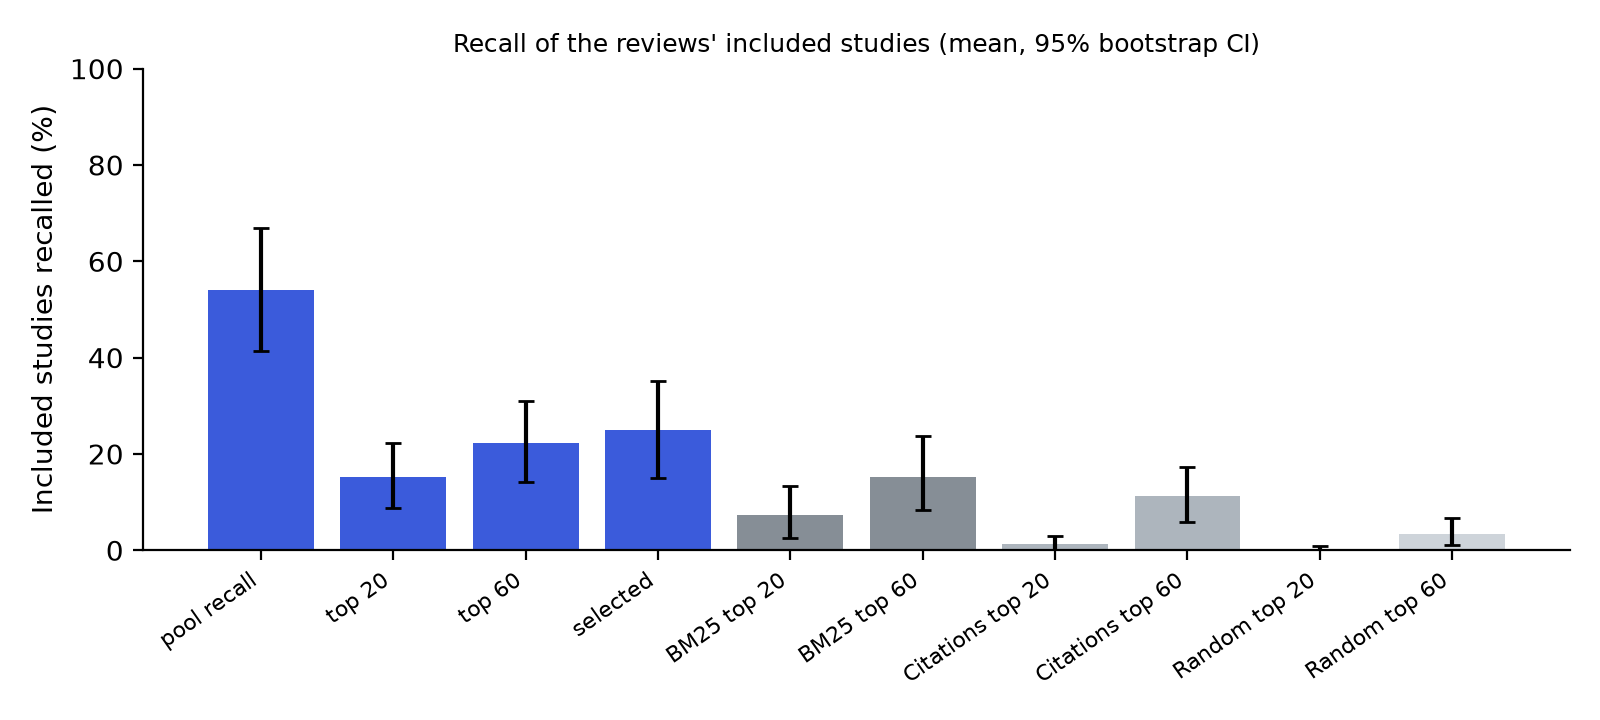
\includegraphics[width=\linewidth]{figures/fig_recall.png}
\caption{Recall of the 22 test reviews' included studies: \tool{}'s candidate pool, the top 20 and top 60 of its
screening order and its selection (blue), and three baselines ranking the same pools (grey). Means with 95\%
bootstrap CIs.}
\label{fig:recall}
\end{figure}

The 100-point score ordered the pools better than each baseline: the top 20 held 15\% of the included studies
against 7\% for BM25 against the question, 1\% for citation count and 0\% at random (top 60: 22\%, 15\%, 11\%, 3\%).
Model screening kept a mean of 87\% of the included studies it saw (median 100\%), with low precision (10\%), as
expected for a step that keeps records unless a criterion is clearly not met. Citation searching and review
reference lists added 15 included studies that no database search returned. The quick-answer mode, which collects
100--170 records per question and selects 20, held 15\% of the reviews' included studies in its pool and 4\% in its
selection: it answers a question quickly but is not a review search.

\subsection{Where included studies were lost}
\label{sec:loss}

Table~\ref{tab:loss} classifies the 538 included studies the systematic-style runs did not select. Eighty per cent
were lost at search. Half of all losses (266) were studies that one of \tool{}'s own PubMed queries matches but that
ranked beyond the 500 records retrieved; one review with 245 included studies accounts for 134 of them. Another 169
were matched by no query. Losses at eligibility (67) and screening (36, of which 27 were eligible but never reached
because of the screening cap and study limit) were smaller.

\begin{table}[t]
\centering
\caption{Where and why the 538 included studies not selected were lost (22 test reviews).}
\label{tab:loss}
\footnotesize
\begin{tabularx}{\linewidth}{>{\raggedright\arraybackslash}Xrr}
\toprule
Stage and reason & Studies & Share \\
\midrule
Search: beyond the retrieval depth (a \tool{} PubMed query matches it) & 266 & 49\% \\
Search: no \tool{} query matches it & 169 & 31\% \\
Eligibility: concept words not matched & 55 & 10\% \\
Screening cap or study limit (eligible, never screened) & 27 & 5\% \\
Eligibility: set aside as a review article by publication type & 10 & 2\% \\
Model screening: a criterion answered ``no'' & 9 & 2\% \\
Eligibility: other (not a research report) & 2 & 0\% \\
\bottomrule
\end{tabularx}
\end{table}

Reading the stored corpora showed three recurring causes. First, selection reads a rule-based parse of the
question so that it does not depend on the model, and where the parse was poor it cost recall: for ``First-line
drugs inhibiting the renin angiotensin system versus other first-line antihypertensive drug classes for
hypertension'', the rules produced the concept ``first-line drugs inhibiting'', and 609 of 640 records were judged
off topic, while the model's plan for the same question named ``renin-angiotensin system inhibitors''. Second, a
question naming a class of interventions (``psychological therapies'', ``inhaled corticosteroids'') was answered by
studies naming its members (cognitive behavioural therapy; fluticasone), which word matching missed when PubMed
mapped the class to a different heading. Third, in 8 of the 9 screening losses the model turned the question's
structure into a required criterion: in ``intralesional treatment versus wide resection'' the comparator became the
criterion ``outcome: wide resection'', and case series of the intervention alone, which the review included, were
screened out.

\subsection{Repeatability and sensitivity}

\emph{Selection given the same records (E2a).} All 44 stored test corpora (22 per mode) reproduced their included
studies, in the same order and with matching content hashes, from their stored records alone, with no network and
no model. Because model screening decisions are stored, this covers the systematic-style selection.

\emph{Model screening of the same records (E2b).} Three repeats of the screening of 1,638 records agreed with each
other on 96--97\% of decisions (Cohen's $\kappa$ 0.91--0.94) and with the original decisions on 90--91\% ($\kappa$
0.80--0.82); the original run screened records in batches in score order and the repeats in sample order, so part
of this difference reflects batch context. Sensitivity on the 117 included studies in the sample was 92\% originally
and 93\% in each repeat. A second model could not be measured: the free models tried were rate-limited upstream.

\emph{Records found (E2c, E2d).} Repeating the searches gave different records: two identical rule-planned repeats
shared a median of 63\% of their records (lowest 24\%), with similar pool recall (34\% and 37\%). The difference came
from sources that did not answer within the time budget in one run, and from citation searching that Semantic
Scholar rate-limited, which adds all or nothing. Model planning raised pool recall from 34--37\% (rules) to 54\%;
re-planning each question three times with the model gave the same concept names (median overlap 1.00) but the
same core PubMed string in only 14 of 66 plans, because the synonyms it adds vary.

\emph{Sensitivity to the score's constants (E3).} Setting each weight or cap to half or one and a half times its value
changed about one of the 20 quick-answer selections (median Jaccard overlap 0.90--0.95) and recall by at most 0.3
percentage points; halving the caps on reviews changed the quick-answer selection most (median overlap 0.57)
without changing recall (Fig.~\ref{fig:sensitivity}). In the systematic-style runs the records the model would
screen were unchanged in most reviews (median overlap 1.00, lowest 0.85).

\begin{figure}[t]
\centering
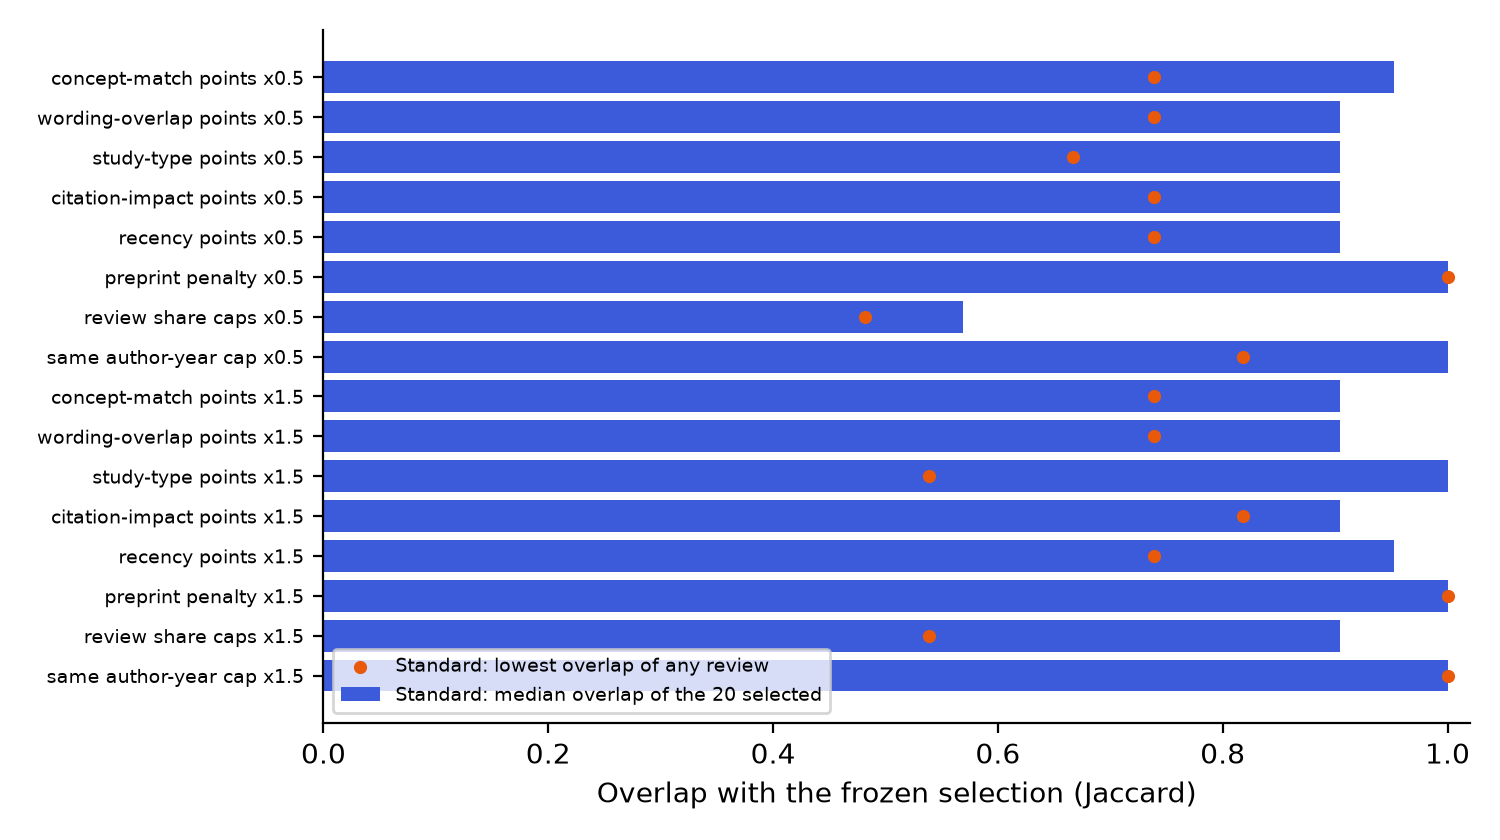
\includegraphics[width=0.85\linewidth]{figures/fig_sensitivity.png}
\caption{Sensitivity of the quick-answer selection to each score weight and cap, set to half and one and a half
times its value: median (bars) and lowest (dots) Jaccard overlap with the frozen selection over the 22 test
reviews.}
\label{fig:sensitivity}
\end{figure}

\subsection{Components and written claims}

\emph{Study type.} With PubMed's publication types removed, the classifier labelled 67\% of 26,114 records
correctly from wording alone; trials had precision 0.88 and recall 0.62, systematic reviews and meta-analyses 0.82
and 0.58, and case reports and narrative reviews were mostly called other primary research. With Semantic Scholar's
own types (2,819 papers) accuracy was 0.78. Because 80\% of the included studies in the test corpora carry PubMed's
own types, which the classifier reads first, these figures apply to the remaining 20\%.

\emph{Duplicate merging.} \PENDING{share of the 100 sampled merges judged to be the same study, by kind of merge}

\emph{Claims in the written synthesis.} Over the 33 model-written analyses, the rule-based checks changed no
narrative and excluded none of 117 structured claims; one narrative needed a corrective retry during generation.
\PENDING{Of the 200 sampled cited sentences, N\% were supported, N\% partly supported and N\% not supported by the
studies they cite (95\% CI); agreement between the two annotators on 50 sentences, Cohen's $\kappa$ = N.}

\section{Discussion}
\label{sec:discussion}

\subsection{Principal findings}

Separating a rule-based, stored selection from the steps where a model helps made \tool{}'s study selection exactly
reproducible from its stored records, while the model's contribution stayed measurable and bounded. Repeating a run
does not give the same records: the model's search plan varies in its synonyms, and databases differ in what they
return on a given day. The corpus turns this from an unknown into a record: it holds what was found, what was
asked, and every decision, so a review can be audited and its selection replayed even when a new search would
differ. The model's screening was highly consistent with itself on the same records ($\kappa$ above 0.9), and the
score's constants could be changed by half without moving recall by more than a third of a percentage point.

On held-out Cochrane intervention reviews, the systematic-style mode found about half of each review's included
studies and selected a quarter. This is far from what a systematic search achieves, and we do not suggest it can
replace one. The loss analysis shows why, and where to improve: four in five lost studies were lost at search, half
of them because they ranked beyond the 500 PubMed records retrieved by queries that do match them. Ranking and
screening, the steps most LLM tools focus on, accounted for less of the loss; the model screen kept 87\% of the
included studies it saw.

\subsection{What the design costs}

Keeping the selection independent of the model has a price, which the evaluation makes visible. Selection reads a
rule-based parse of the question, and where the parse was poor (a verb or participle joined to a concept, a class
named where studies name its members) included studies were judged off topic even though the model's search plan
had named the concept correctly. Two of 22 reviews selected nothing for this reason. In the evaluation each question
was the review's title, run with the default protocol and no person confirming it; in \tool{}'s guided review the
user sees and edits the parsed concepts before anything is searched, which is the intended remedy. The recall
reported here is therefore that of the tool used without that step.

\subsection{Comparison with other work}

Tools that rank records for screening are usually evaluated on a fixed set of records, by the work saved before a
target recall is reached \citep{omara2015using,vandeschoot2021open}; that measures ranking and not search. Studies of
LLM screening report agreement with human decisions on given records \citep{guo2024automated,khraisha2024can}, and
studies of LLM-written search strings report precision and recall of the strings \citep{wang2023can}. Our evaluation
follows the whole path from question to selected studies against the included studies of published reviews, and
attributes each lost study to a stage, which is what a reviewer needs to judge where the tool can be trusted. The
repeatability problem reported for a commercial LLM assistant \citep{elicit2025repeat} is addressed here not by
making the search deterministic, which the evidence suggests is not possible with live databases and models, but by
storing what each run found and making the selection a replayable function of it.

\subsection{Implications}

For tool developers, the largest gains lie in retrieval depth and query sensitivity rather than ranking: deeper
paging of the queries that already match, and better handling of intervention classes (for example through
pharmacological-action headings). For users, the quick-answer mode of such tools, which held 4\% of a review's
included studies, should not be mistaken for a literature search, and a systematic-style result should be read with
its pool recall in mind. Consistent with recent guidance on AI in evidence synthesis \citep{raise2026}, \tool{}
labels its results, shows its search strings and counts, keeps every screening decision open to the user's override
with a recorded reason, and marks a review that synthesised fewer than all its eligible studies as not complete.

\subsection{Limitations}
\label{sec:limits}

The benchmark covers Cochrane intervention reviews published before mid-2019, and recall may differ for other
questions, fields and review types. Cochrane reviews search sources \tool{} does not (Embase, CENTRAL, trial
registers, grey literature) and screen full texts, so their included studies are a demanding reference standard for
a tool limited to open databases. One model was used throughout; a second screening model could not be measured,
and the model screened titles and abstracts truncated to 420 characters. Search and selection were developed on the
development reviews and frozen after the systematic-style test results had been seen (no change was made to them on
account of those results). Repeats of the record search were made with rule-based planning only. Risk-of-bias
suggestions were not compared with published judgements, because the benchmark does not include them and few
included studies have open full text; they are reported as exploratory. \PENDING{claim-accuracy limitation: single
main annotator, abstracts only, sample of 200 of 881 sentences}. Finally, the software and this evaluation were built
by a single author with extensive AI assistance (Section~\ref{sec:ai}); every result is produced by scripts from
stored runs, and the code, corpora and results are public so that they can be checked.

\subsection{Future work}

Planned work includes deeper and more sensitive searches, a second screening model, a comparison of the risk-of-bias
suggestions with published judgements, and a study of the guided review with reviewers. A count-based evidence gap
map, which fills a grid of interventions by outcomes with dated database counts rather than with the selected
studies \citep{snilstveit2016evidence}, has been added to \tool{} since the evaluation and will be evaluated
separately against published evidence gap maps.

\section{Conclusion}

Making study selection a replayable function of stored records, with a bounded and recorded role for the model,
makes LLM-assisted study selection auditable and reproducible without requiring live searches or models to behave
deterministically. Measured honestly against Cochrane reviews, such a tool finds about half of a review's included
studies, and most of what it misses is lost at search, which points to where these tools should improve and confirms
that they support, rather than replace, a systematic search.

\section*{Data and code availability}
\label{sec:availability}

The source code is available at \url{https://github.com/mbsai/citelume} under the MIT licence; the code evaluated is
tagged \path{eval-freeze-2.5}, and version \TODO{v1.0.0} is archived at \TODO{Zenodo DOI}. The evaluation archive
(\TODO{Zenodo DOI}) contains the pre-registered protocol and its amendments, the benchmark and its split, the freeze
record, every results table and figure, and for each evaluation run the stored corpora, raw search output, results
and run records, with a checksum manifest; the recall tables can be reproduced from it without searching again. The
corpora hold bibliographic records as the databases returned them; abstracts remain the copyright of their
publishers and are included for reproducibility only. No API keys, imported database exports or uploaded PDFs are
included. A public demonstration is available at \url{https://citelume-976737283006.us-central1.run.app}
\TODO{label as research version}.

\section*{Declaration of generative AI and AI-assisted technologies in the writing process}
\label{sec:ai}

\TODO{Check against the journal's policy and your own account; adapted from docs/AI\_USAGE.md.} The author conceived,
directed and is responsible for this work. Most of the software, the analysis scripts and the text of this
manuscript were drafted by an AI coding assistant (Claude, Anthropic, used through Claude Code) under the author's
direction, session by session from a written plan. The author made every design and evaluation decision (including
the pre-registration, the benchmark, the freeze and every change to the evaluation design), and reviewed and edited
the manuscript. The annotation of claims and merged records was done by people. Every number reported is produced
by scripts from the stored runs, and the code and data are public. The AI tool is not an author.

\section*{Funding}
\TODO{State funding, or: This research did not receive any specific grant from funding agencies in the public,
commercial, or not-for-profit sectors.} Model use for the evaluation cost under 3~USD in total.

\section*{Declaration of competing interest}
\TODO{The author declares no competing interests -- confirm.}

\section*{CRediT authorship contribution statement}
\textbf{Bhargava \TODO{family name}:} Conceptualization, Methodology, Software, Validation, Formal analysis,
Investigation, Data curation, Writing -- original draft, Writing -- review \& editing, Visualization.
\TODO{add any co-authors and annotators who qualify}

\section*{Acknowledgements}
We thank the organisers of the CLEF eHealth Technology Assisted Review track for making their data available.
\TODO{annotators, if not authors}

\section*{Supplementary material}
S1: PRISMA-S checklist for the search methods (\path{supplement/prisma_s.tex}). S2: the evaluation protocol and
its amendments (\path{eval/PROTOCOL.md}). S3: per-review results and the loss-by-stage table
(\path{eval/results/6_test.md}, \path{6_test_loss_by_stage.md}). \TODO{TRIPOD-LLM checklist, if the journal
asks for it}


\bibliographystyle{elsarticle-harv}
\bibliography{references}

\end{document}
